\documentclass{lutmscthesis}[2010/09/22]

% ---
% BEGIN SETTINGS
% ---
\usepackage[latin1]{inputenc}
\usepackage[T1]{fontenc}
\usepackage[english,finnish]{babel}

\usepackage{times}

\usepackage{setspace}
\usepackage{verbatim}
\usepackage[intlimits]{amsmath}

% Ensure figure captions are below and table captions are above the content.
\usepackage{float}
\floatstyle{plain}\restylefloat{figure}
\floatstyle{plaintop}\restylefloat{table}

\usepackage[pdfborder={0 0 0}]{hyperref}

 % Graphics search path
\graphicspath{{images/}}

\newcommand{\vect}[1]{\boldsymbol{#1}}
\newcommand{\matr}[1]{\boldsymbol{#1}}
\newcommand{\diag}[1]{\mathrm{diag}(#1)}
\newcommand{\iprod}[1]{\left\langle #1 \right\rangle}
\newcommand{\me}{\mathrm{e}}
\newcommand{\mi}{\mathrm{i}}
\newcommand{\md}{\mathrm{d}}
\newcommand{\sse}{{}} %\mathrm{SSE}}
\newcommand{\trace}{\mathrm{Tr}\:}
\newcommand{\frp}[2]{{}^\mathrm{#1}\vect{#2}}
\newcommand{\frs}[3]{{}^\mathrm{#1}#2_\mathrm{#3}}
\newcommand{\frv}[3]{{}^\mathrm{#1}\vect{#2}_\mathrm{#3}}
\newcommand{\frm}[3]{{}^\mathrm{#1}\matr{#2}_\mathrm{#3}}
\newcommand{\colvec}[2]{\genfrac{[}{]}{0pt}{1}{#1}{#2}}
\newcommand{\relphantom}[1]{\mathrel{\phantom{#1}}}

% Tables
\usepackage{array}
\usepackage{multirow}
\newcolumntype{L}[1]{>{\raggedright\let\newline\\\arraybackslash\hspace{0pt}}m{#1}}
\newcolumntype{C}[1]{>{\centering\let\newline\\\arraybackslash\hspace{0pt}}m{#1}}
\newcolumntype{R}[1]{>{\raggedleft\let\newline\\\arraybackslash\hspace{0pt}}m{#1}}

% Code
\usepackage{listings}
\usepackage{xcolor}
\renewcommand{\lstlistingname}{Listing}

\colorlet{punct}{red!60!black}
\definecolor{background}{HTML}{FFFFFF}
\definecolor{delim}{RGB}{20,105,176}
\colorlet{numb}{magenta!60!black}

\lstset{frame=single,
  language=Python,
  aboveskip=10mm,
  belowskip=0mm,
  captionpos=b,
  basicstyle={\footnotesize\ttfamily},
  numbers=left,
  numberstyle=\footnotesize\ttfamily,
  breaklines=true,
  frame=lines,
  stepnumber=1,
  showstringspaces=false
}

\lstdefinelanguage{json}{
    basicstyle=\footnotesize\ttfamily,
    numbers=left,
    numberstyle=\footnotesize\ttfamily,
    stepnumber=1,
    numbersep=8pt,
    showstringspaces=false,
    breaklines=true,
    frame=lines,
    backgroundcolor=\color{background},
    literate=
     *{0}{{{\color{numb}0}}}{1}
      {1}{{{\color{numb}1}}}{1}
      {2}{{{\color{numb}2}}}{1}
      {3}{{{\color{numb}3}}}{1}
      {4}{{{\color{numb}4}}}{1}
      {5}{{{\color{numb}5}}}{1}
      {6}{{{\color{numb}6}}}{1}
      {7}{{{\color{numb}7}}}{1}
      {8}{{{\color{numb}8}}}{1}
      {9}{{{\color{numb}9}}}{1}
      {:}{{{\color{punct}{:}}}}{1}
      {,}{{{\color{punct}{,}}}}{1}
      {\{}{{{\color{delim}{\{}}}}{1}
      {\}}{{{\color{delim}{\}}}}}{1}
      {[}{{{\color{delim}{[}}}}{1}
      {]}{{{\color{delim}{]}}}}{1},
}


% ---
% END SETTINGS
% ---

% ---
% Thesis information
% ---
\title{Software for Transport Accessibility Analysis: The Case of Moscow}
\author{Tikhon Belousko}
\Major{Degree Program in Intelligent Computing}
\Faculty{School of Engineering Science}
\Doctype{}
\Keywords{web-based maps, GIS, transport accessibility, vector tiles}
\Supervisors{Assoc. Prof. Arto Kaarna\\ Sen. Lec. Vitaly Bragilevsky}
\Examiners{Assoc. Prof. Arto Kaarna\\ Sen. Lec. Vitaly Bragilevsky}
\AcceptDate{January 1\textsuperscript{st}, 2016} % TODO
\SignDate{July 3\textsuperscript{rd}} % TODO
\Year{2016}
\addtostats{, 2 thingy, 3 stuff}


% ---
% Document
% ---
\begin{document}
\selectlanguage{english}

% ---
% Title
% ---
\maketitle
\newpage


% ---
% Preface and Abstract
% ---
%!TEX root = ../thesis.tex
\begin{abstract}

In this thesis the process of building a software for transport accessibility analysis is described.
The goal was to create a software which is easy to distribute and simple to use for the user without
particular background in the field of the geographical data analysis. It was  shown that existing
tools do not suit for this particular task due to complex interface or significant rendering time.
The goal was accomplished by applying modern approaches in the process of building web applications
such as maps based on vector tiles, FLUX architecture design pattern and module bundling. It was
discovered that vector tiles have considerable advantages over image-based tiles such as faster
rendering and real-time styling.

\end{abstract}
%!TEX root = ../thesis.tex

\begin{preface}
First, I would like to thank my supervisors -- Vitaliy Bragilevsky and Arto Kaarna for
help and support in course of choosing topic and writing this thesis.

Second, I am happy that I was able to do this work in Lappeenranta University of Technology,
where I had personal space to work any time without being disturbed. I feel lucky for
working in Machine Vision Laboratory where people created the warmest atmosphere to work in.

Finally, I would like to thank Vadim Smakhtin and Eduard Haiman for providing me with topic
for research. I think I learned a lot from this collaboration.


\

Lappeenranta, April 19th, 2016
\end{preface}

% ---
% Table of Contents
% ---
\renewcommand\refname{REFERENCES}
\renewcommand\contentsname{CONTENTS}
\newpage
\tableofcontents

% ---
% Chpaters
% ---
\setlength{\parskip}{3ex}
%!TEX root = ../thesis.tex
\section{ INTRODUCTION }

\subsection{ Background }
% In recent years, there have been many papers describing ...

\subsection{ Objectives and Delimitations }
The objective of this thesis is to design a software for transport accessibility analysis
which can used for by people without special background in the field. Another important
requirement is simplicity of the distribution. Thus, software had to be implemented
as a web service which can accessed by any modern browser. The performance of the interface
is crucial, hence the user would not be irritated or confused. The delays related to the processing,
rendering and data transfer should be minimized or illuminated completely.

It is expected that the program will be useful for various groups of actors which
were divided in 5 categories such as state institution, logistics, real estate, science
and citizens. All categories with description are listed in Table~

\begin{table}[ht]
  \renewcommand{\arraystretch}{1.5}
  \centering
  \footnotesize
  \begin{tabular}{p{4cm} p{2.5cm} p{2.5cm} p{1.5cm} p{2.2cm}}
    \hline
    \textbf{State Institutions} & \textbf{Logistics} &\textbf{Real Estate}
    & \textbf{Science} & \textbf{Citizens} \\
    \hline

    Department of Complete Overhaul of Moscow &
    Trading companies &
    Realtors &
    Mapping &
    Tourists \\

    %%

    Department of Culture of Moscow &
    Logistics companies &
    Post officers &
    Ecology &
    Travelers  \\

    %%

    Department for Housing, Utilities and Amenities &
    &
    Collector Logistics &
    Sociology &
    Guest workers \\

    %%

    Department for Transport and Road Infrastructure Development
    &
    &
    Political science &
    \\

    %%

    Department for Urban Development and Construction &
    &
    &
    &
    \\

    \hline
  \end{tabular}

  \caption{Potential actors.}
  \label{tab:actors}
\end{table}

\subsection{ Structure of the Report }
The paper is divided into $N$ main sections...
\section{ OVERVIEW }

\subsection{ GIS Tools for Accessibility Analysis }
\subsection{ Modern Web-based Maps }
\subsection{ Data Formats }
\subsubsection{ GeoJSON }
\subsubsection{ MBTiles }
\subsubsection{ Protocol Buffers }



%!TEX root = ../thesis.tex
\section{SOFTWARE REQUIREMENTS SPECIFICATION}

The software development process starts with writing a software requirements specification (SRS)
so that
it serve as an agreement between client and contractor about the set of the
features which need to be implemented. Another important purpose of this document
is to create understanding of the features with higher and lower priority, thus developer
would know what should be implemented in the first version of the product and what could
be added later.

In this section the simplified version of the SRS will be presented which includes description
of the user interface, operating environment, and set of system features with detailed
explanation.

\subsection{Graphical User Interface}

The interface design was provided by Mathrioshka LLC, which includes set of different states
of the application with small description provided. The interface should have been implemented
to work in browser with use of HTML5 standard. The whole program should be implemented
as single page application, which means that all changes in the state of the application
happen without page reload. The interface have to be responsive and support screen sizes
starting from $800 \times 600$ pixels.

The manipulation of the data within the application is performed utilizing main control elements.
Most important elements are listed below:

\begin{enumerate}
  \item Mode selector is needed for switching from general overview to location-wise analysis and
  located in the left bottom corner of the screen.

  \begin{figure}[ht]
    \centering
    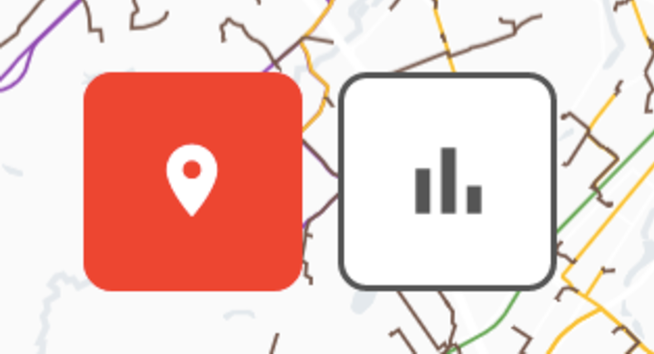
\includegraphics[width=0.33\textwidth]{mode-selector.pdf}
    \caption{Mode selector.}
    \label{pic:mode_selector}
  \end{figure}

  \item Overview mode selector switches different types of overview analysis tools. For some
  views it has embedded slider used for filtering. The component is positioned on the right
  side of the screen.

  \begin{figure}[ht]
    \centering
    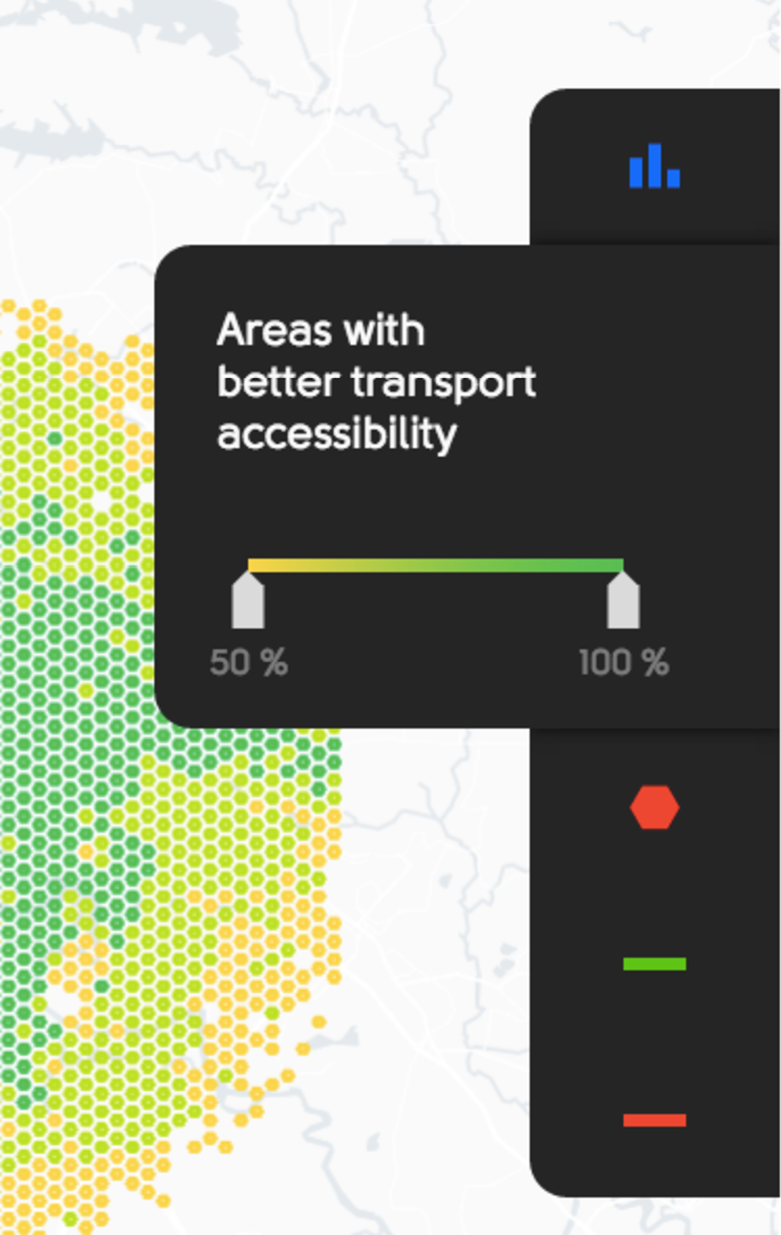
\includegraphics[width=0.25\textwidth]{overview-mode.pdf}
    \caption{Overview mode selector.}
    \label{pic:overview_selector}
  \end{figure}

  \item Transport filter is a set of checkboxes where every checkbox represent certain
  type of transport. This component is placed on top of the screen.

  \begin{figure}[ht]
    \centering
    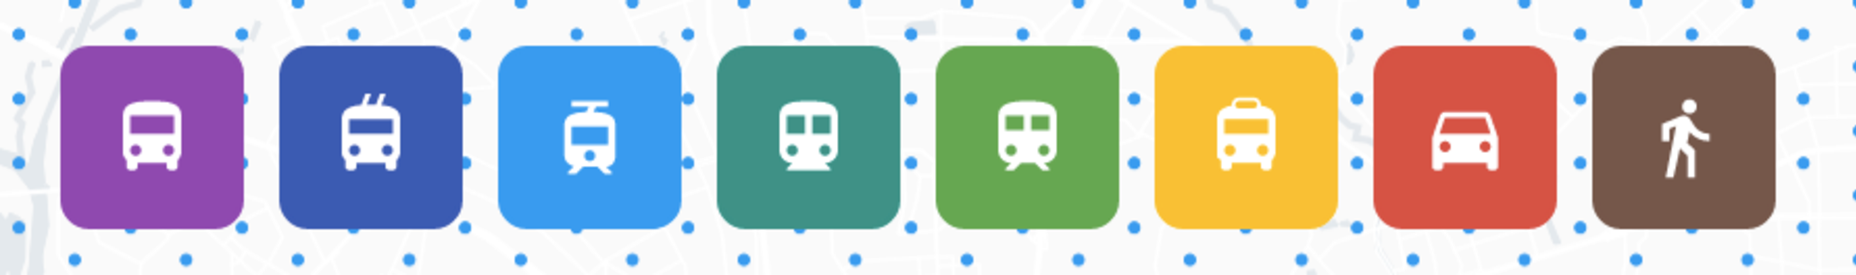
\includegraphics[width=0.8\textwidth]{transport-filter.pdf}
    \caption{Transport filter.}
    \label{pic:transport_filter}
  \end{figure}

  \item Current location indicator shows what point is selected on the map at this moment and
  also allows to clear current selection. The component is located on the right side of the window.

  \begin{figure}[ht]
    \centering
    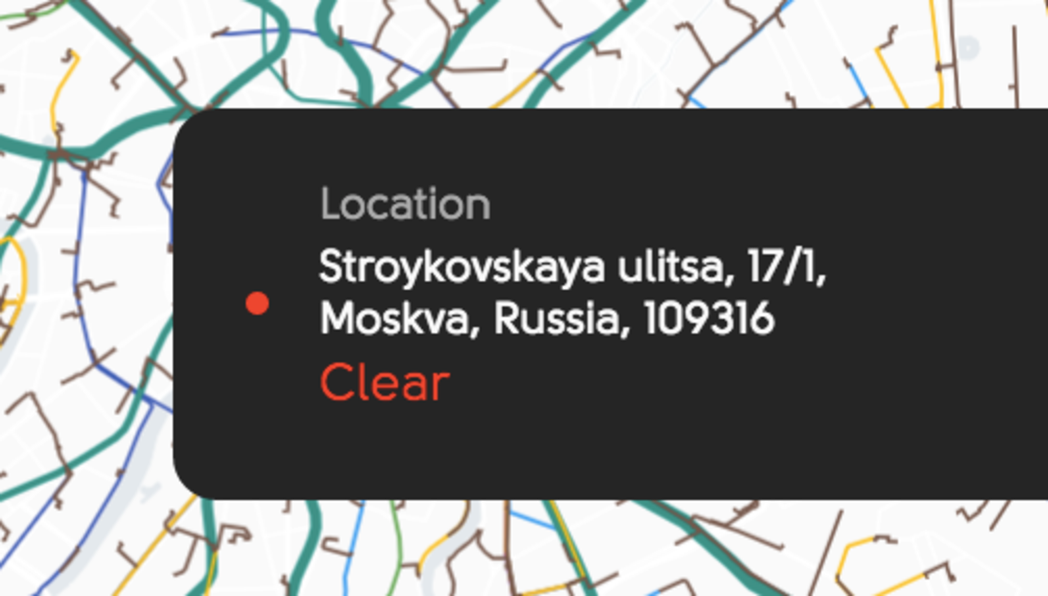
\includegraphics[width=0.3\textwidth]{location-selector.pdf}
    \caption{Current location indicator.}
    \label{pic:transport_filter}
  \end{figure}

  \item Map is the most important element of the interface which is presented on every screen
  of the application the only thing that changes is the content of the map.
  This component can show points, areas, routes and also provides functionality for
  selecting particular locations for analysis.

  \begin{figure}[ht]
    \centering
    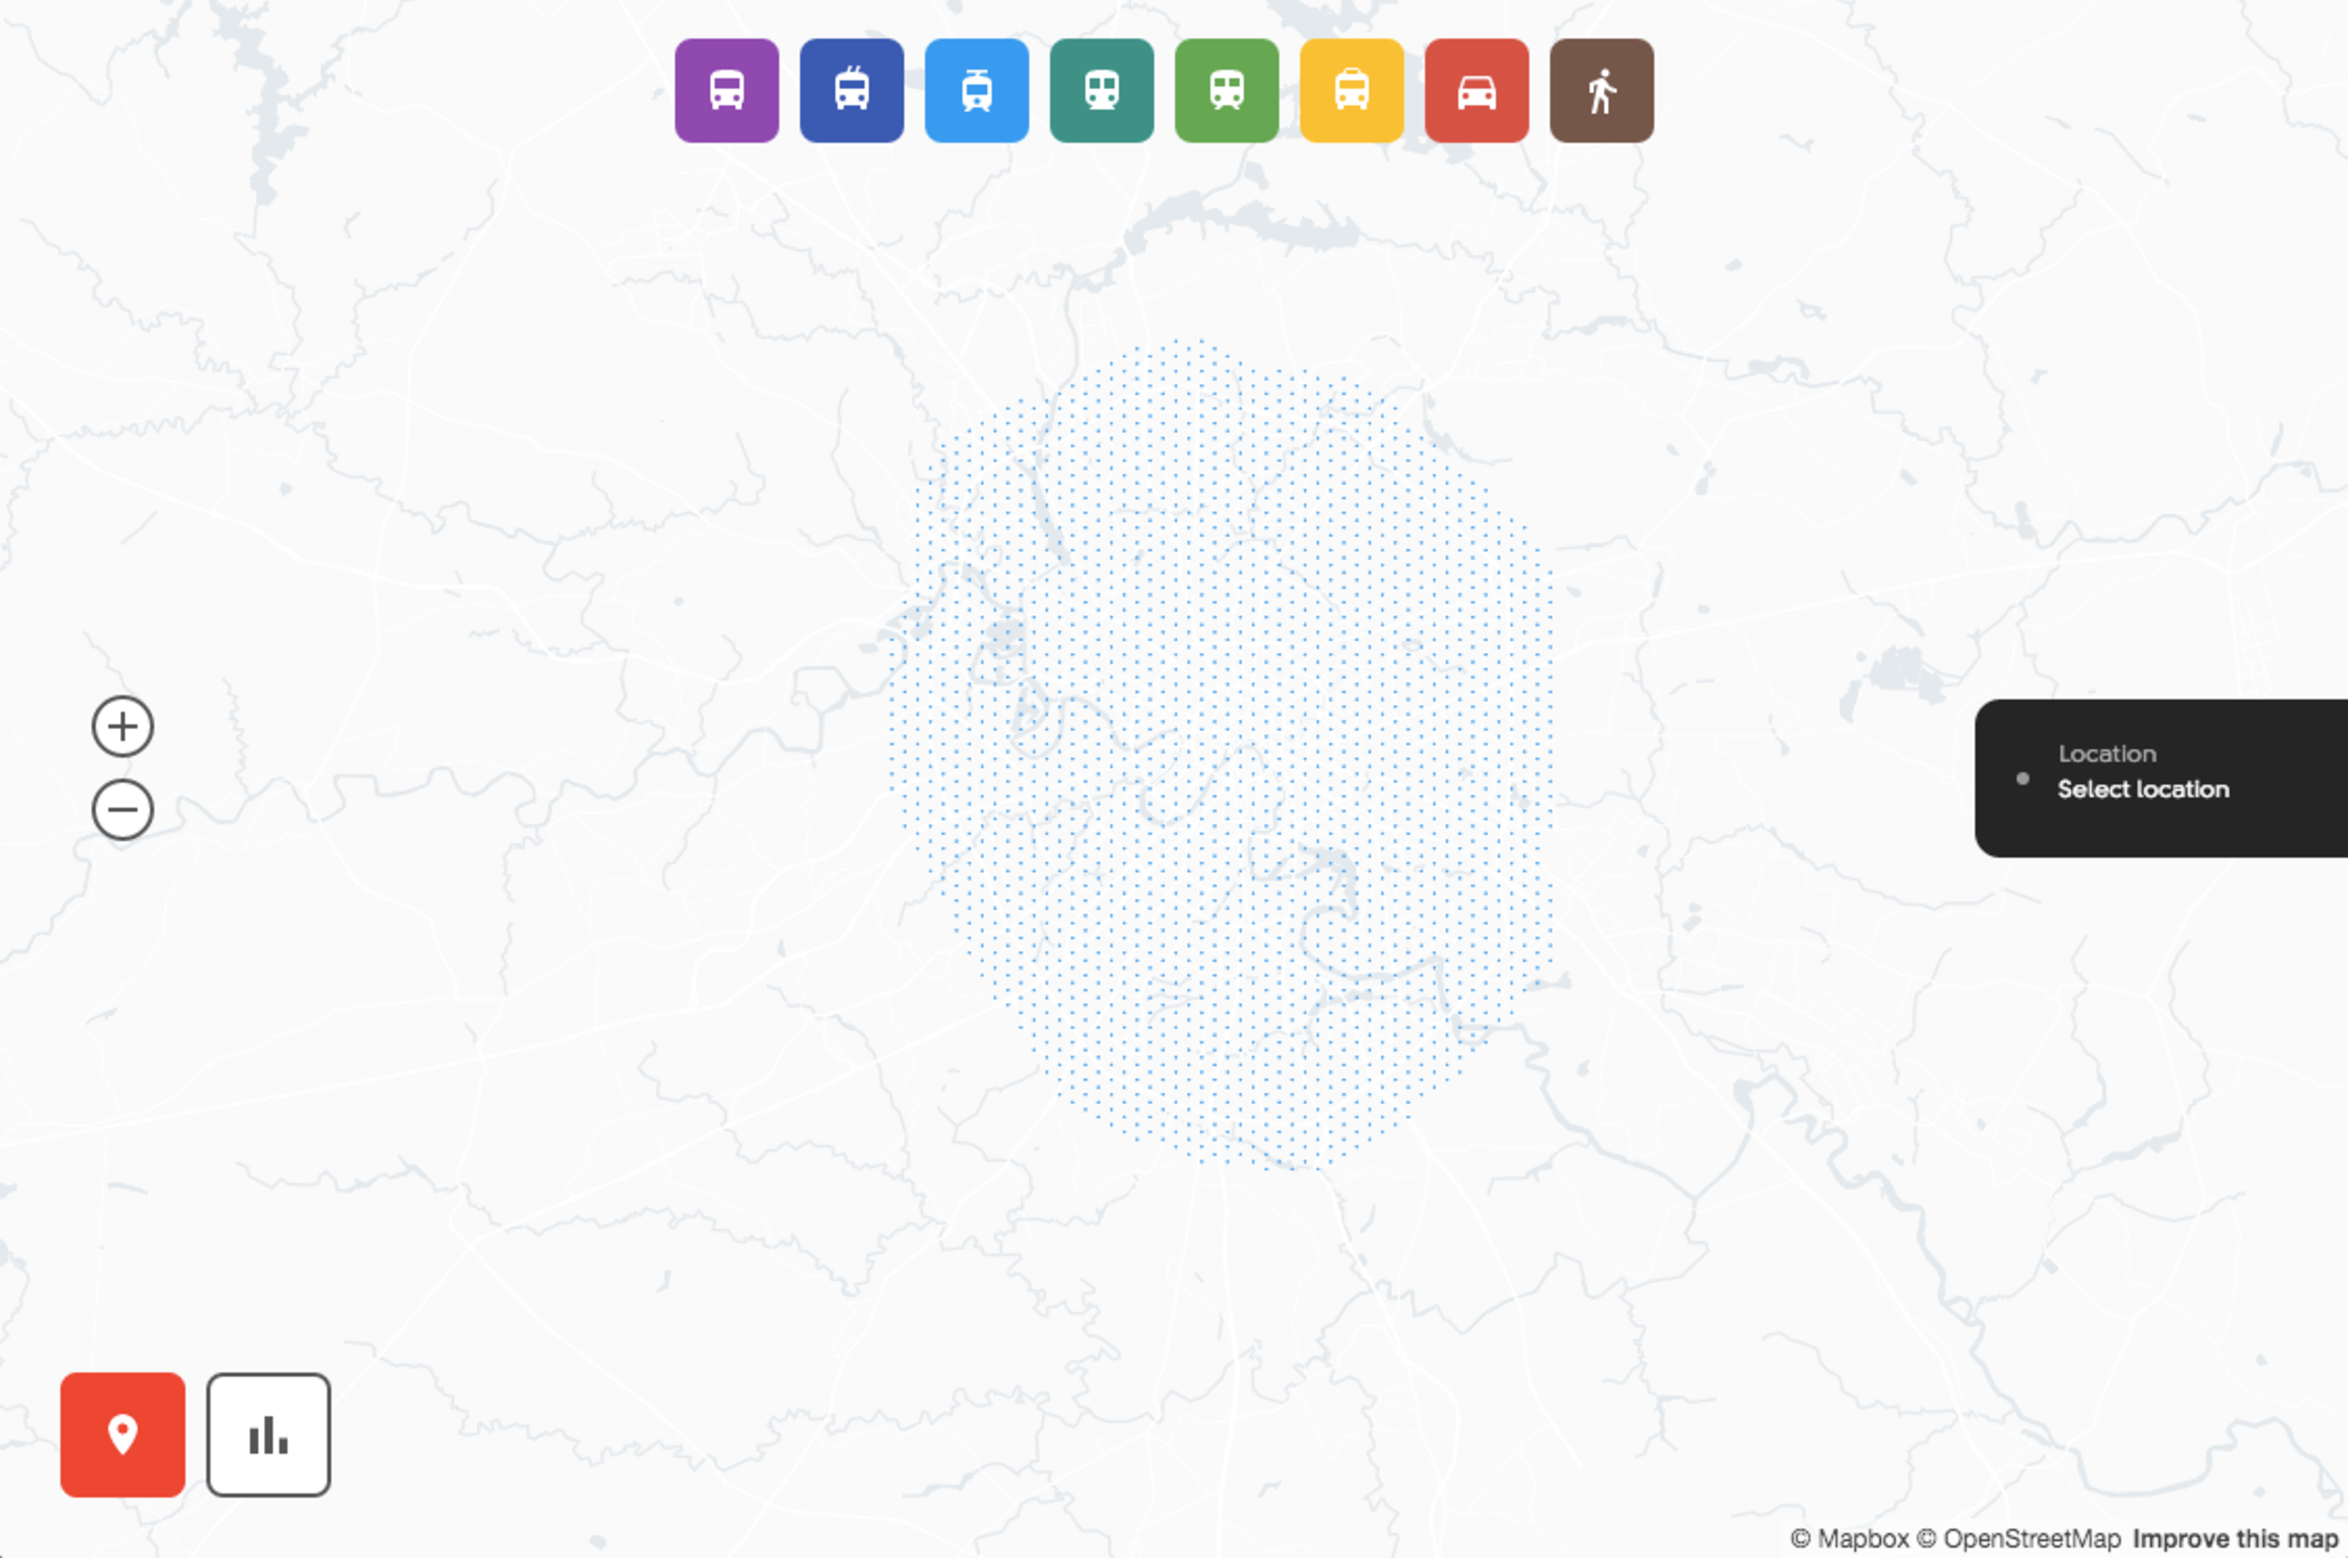
\includegraphics[width=0.80\textwidth]{map.pdf}
    \caption{Map.}
    \label{pic:map}
  \end{figure}

\end{enumerate}

\subsection{Operating Environment}

The software is developed on x86 based computer using Mac OS X 10.11 operating system. The
computer hardware is featured 8~GB 1600~MHz DDR3 RAM and 1.6 GHz Intel Core i5 processor.
The client should operate on any system which is able to install browsers like Google Chrome~49.0,
Safari, Firefox or Microsoft Edge. Hence it works well on Windows, Mac OS X and Linux. As for the
server, it was tested to work on Ubuntu~14.04 and 512~Mb~RAM. Running the server side on Windows
was not tested.

\subsection{System Features}

\begin{description}
  \item[Use case 1:] Hello there this is the first use case... bla bla bla...
\end{description}
%!TEX root = ../thesis.tex

\section{ Architecture }
\subsection{ Client }

The first significant part of the application is the client which will
be the interface for the user to manipulate map and data. The core functionality of the client
is follows:

\begin{enumerate}
  \item Panning and zooming map.
  \item Selecting a point on the map to build a whole graph of
  the routes needed to move from selected point to all other points of the city. All of the routes
  are parametrized by color and width. This parameters are calculated utilizing information
  about transport type specified in this point and the coefficient which is defined as number of
  times this particular line is used in all of the directions calculated from this point.
  \item Showing prevailing transport in all points of the grid. Prevailing transport is defined
  by calculating total time spent in each transport type. The maximum of all of the values will
  be taken as prevailing.
  \item Showing fastest and slowest roads. The map should also have interactive slider
  which will be used to filter roads within particular speed range.
  \item Showing most accessible points on the grid. The transport accessibility coefficient of the
  point can be defined as total time spent in a transport while moving from selected point to all
  other points. All of the values after that scaled to be between 0 and 1. This view should also
  have a filter by transport accessibility coefficient.
\end{enumerate}

For the reason of the easy distribution it was selected to use browser based client. Thus
client is implemented as single-page web application, which should support all modern browsers such
as Safari, Google Chrome, Firefox, Microsoft Edge 13.

\subsection{ RESTful Server }

For serving data to the client it was selected to utilize RESTful~\cite{rest:wiki} architectural
style, which represents HTTP approach to read, update and delete data. Due to the fact, that our
application will only read data and not modify it, then we will only need to describe all of
the end-points for data access where data will be encoded in GeoJSON~\cite{geojson:spec}.
For our application following end-points were selected:

\begin{itemize}
  \item \textbf{\texttt{GET /points}} \\
  The returned points are described as FeatureCollection of points with following properties
  \begin{itemize}
    \item \textbf{name} is a string;
    \item \textbf{id} is a unique identifier of the point encoded as string;
    \item \textbf{prevalingTransport} could be \mbox{``BUS''}, \mbox{``TROLLEYBUS''},
    \mbox{``TRAM''}, \\ \mbox{``SUBWAY''}, \mbox{``COMMUTER\_TRAIN''}, \mbox{``SHARE\_TAXI''},
    \mbox{``DRIVING''}, \\ \mbox{``WALKING''}.
    \item \textbf{accessibility} is a floating number in range from 0 to 1.
  \end{itemize}

  \begin{verbatim}
{
  "type": "FeatureCollection",
  "features": [
    "type": "Feature",
    "geometry": [0,0],
    "properties": {
      "id": 0,
      "name": "Location Name",
      "prevailingTransport": "SUBWAY",
      "accessibility": 0.6
    }
  ]
}
  \end{verbatim}

  \item \textbf{\texttt{GET /lines?point\_id}}
  This endpoint is parametrized by point\_id which means that if point id is presented
  then the client will receive only those lines which are associated with specified point.
  On the other hand, if no point id is not specified all lines are returned.

  The properties of the lines can be describe as follows:
  \begin{itemize}
    \item \textbf{id} is a unique identifier of the line encoded as string;
    \item \textbf{travelMode} is on of the \mbox{``BUS''}, \mbox{``TROLLEYBUS''},
    \mbox{``TRAM''}, \\ \mbox{``SUBWAY''}, \mbox{``COMMUTER\_TRAIN''}, \mbox{``SHARE\_TAXI''},
    \mbox{``DRIVING''}, or \\ \mbox{``WALKING''}.
    \item \textbf{weight} number of times this line was used in all of the routes across all of
    the directions' set.
    \item \textbf{duration} time needed to travel this line in seconds.
    \item \textbf{distance} total length of this line in meters.
  \end{itemize}

  \begin{verbatim}
{
  "type": "FeatureCollection",
  "features": [
    "type": "Feature",
    "geometry": [[0,0], [0,0]],
    "properties": {
      "id": 0,
      "width": 1,
      "weight": 200
      "duration": 100,
      "distance": 400,
      "travelMode": "BUS"
    ]
  }
}
  \end{verbatim}
\end{itemize}

It is important to note that we could also add such filtering parameters as \texttt{speed} and
\texttt{travelMode}, but it was revealed during set of experiments that
filtering on server side can take significant amount of time which is up to few
hundreds seconds. Hence, this parameters were dropped and filtering is performed on the client.

Suggested architecture implies that client will perform rendering using GeoJSON data, although
it was investigated that for our purposes rendering becomes rather slow and after series of
optimizations the best rendering time was close to 3 seconds. The next improvement to the
current scheme will be adding tile server which can significantly speed up rendering time.

\subsection{ Tile Server }
Graphical map tiles are usually rectangular images in raster or vector format. Most of the popular
map library providers utilize tiles~\cite{google:tiles, mapbox:tiles} for rendering their maps.
Raster tiles are basically images which do not allow to change color of roads and landscapes.
In contrast, vector tiles are not just images but structures which contain geometries and
metadata such as roads, rivers, places in special compact format. Vector tiles only rendered when
requested by the client.

There are several benefits of using vector tiles. The first, advantage is small size of the tiles,
which allows rendering of high resolution and caching. The second advantage is an ability to change
style of the layers: adjust colors of the geometry, line width, set borders to polygons,
set background patterns. Finally, maps based on vector tiles allow smooth transitions between
zoom levels. Although, the cost of usage of the vector tiles is the lack of
compatibility with older browsers. At the moment most of the libraries demand WebGL support and
Mapbox GL JS does not support Internet Explorer below 9-th version.







%!TEX root = ../thesis.tex

\section{IMPLEMENTATION}

% ---
% Pre-processing
% ---
\subsection{Data Pre-processing}
The work started by preparing the data so servers could work with it the most efficient way. This
section is devoted to the description of the initial data and how it was processed. The section
also involves comparison of deferent approaches of data structuring, their comparison and
summarizing of the results.

\subsubsection{Description of the Raw Data}
The provided original data is collected using Google Directions API~\cite{google:directions}
applying following algorithm. First, on top of the city the grid of points was constructed
using WGS~84~\cite{wiki:wgs} coordinate system. Second, for every pair of points the
directions were calculated using HTTP request to the API. Returned data is encoded in JSON
format written to a text file. As result raw data is a
text file where every line is a JSON object received from Google Directions API. The process
of data collection is demonstrated on Figure~\ref{pic:collecting_data}.

\begin{figure}[ht]
  \centering
  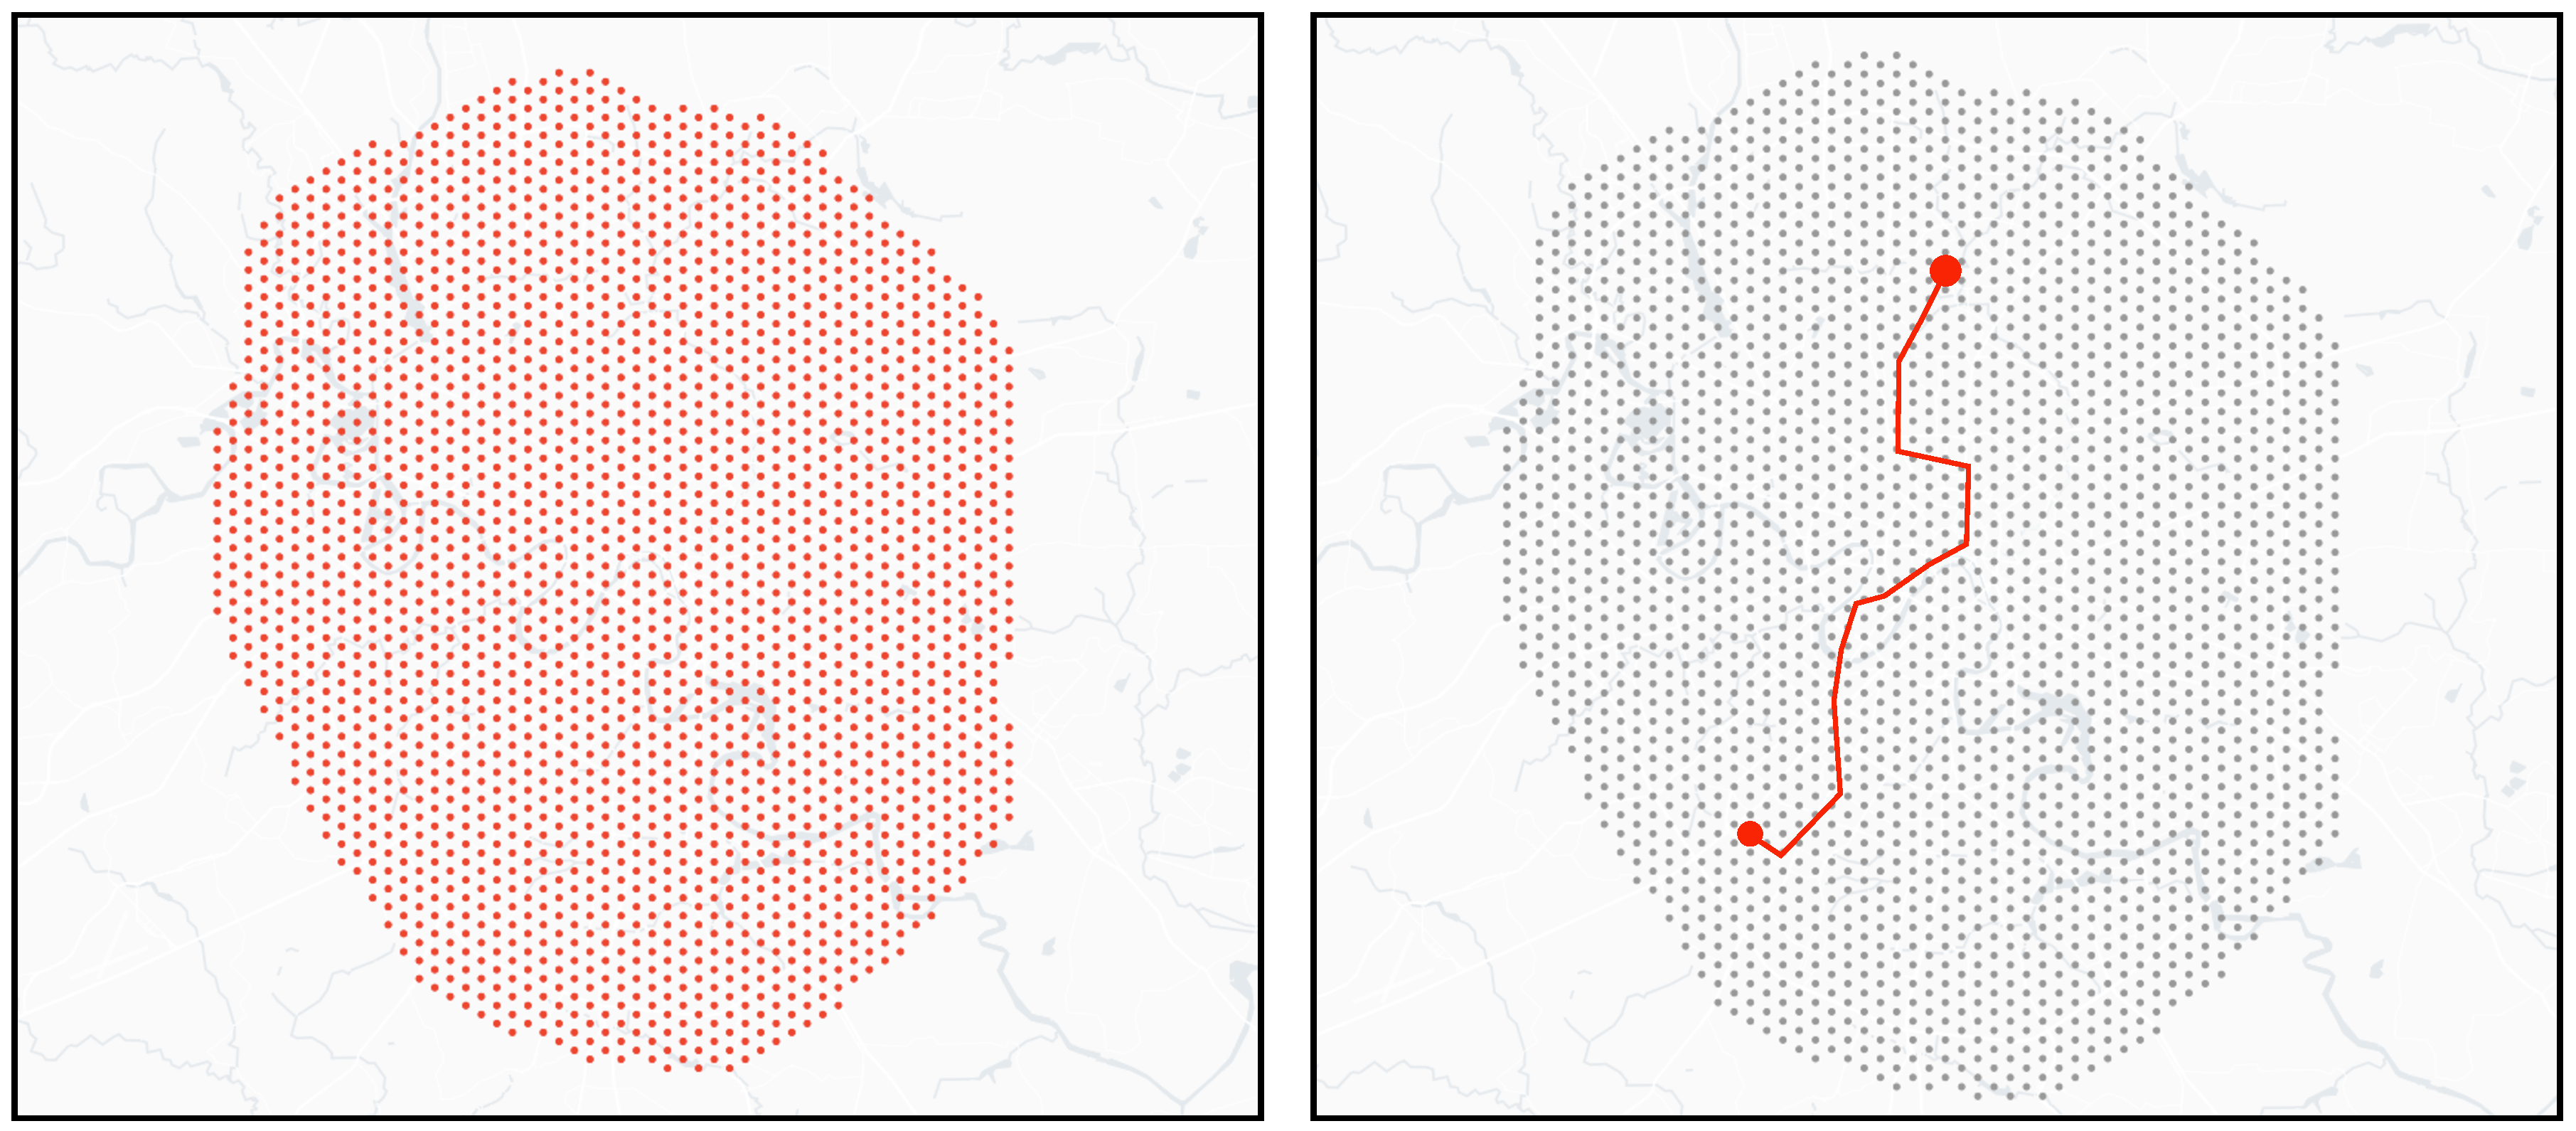
\includegraphics[width=1\textwidth]{data-collection.pdf}
  \caption{The process of the collecting data.}
  \label{pic:collecting_data}
\end{figure}

In fact there is also meta information such as object id, job status, waypoints order,
warnings, but if we simplify and leave only important fields that we will need in pre-processing
step, then JSON object could look like this:

\begin{lstlisting}[language=json, caption=Google Directions API simplified response example,
      label={lst:google_response}]
{
  "start_lat": 55.726497,
  "start_long": 37.338183,
  "end_lat": 55.886619,
  "end_long": 37.579683,
  "data": {
    "routes": [{
      "legs": [{
        "distance": { "text": "45.1 km", "value": 45093 },
        "end_address": "Novgorodskaya ulitsa...",
        "start_address": "Razdorovskaya, Romashkovo...",
        "steps": [{
          "travel_mode": "DRIVING",
          "polyline": { "points": "wicsI{u{bFs@rDC" },
          "distance": { "text": "4.2 km", "value": 4166 },
          "duration": { "text": "7 mins", "value": 438 }
        }, ... ]
      }, ... ]
    }, ... ]
  }
}
\end{lstlisting}

As been be seen from simplified response example, the object contains coordinates of the
start and end point, array routes which consists of \texttt{legs}. \texttt{Legs} are parts of the
route between waypoints. Since in our queries we do not have middle waypoints, the routes array will have
only one element in all cases. Each leg contains total distance information about start and end
location. Also inside \texttt{legs} there is \texttt{steps}, each step is a part of route
which can be described by single command and type of transport, for example ``move forward by bus''
is clearly a step. Step keeps information about its distance and duration which will be needed
to complete this step. Other important things are \texttt{travel\_mode} which indicates what
type of transport is used in this step and \texttt{polyline} which is essentially a set points
of points encoded using lossy Google's algorithm which converts array of float numbers first
to binary representation, then to decimal integers and finally to string using ASCII
codes~\cite{google:polyline}.

\subsubsection{Extracting Points}
The data collection was initiated before by Mathrioshka, thus the first task was extracting
grid points from the raw data. This step was performed utilizing set script written in Python, which
is reading file line by line and extracting starting location point from the data. The
idea of the algorithm is presented in Listing~\ref{lst:points_extraction}. As can be seen from
the listing, Geohash~\cite{wiki:geohash} standard was used to prevent repetitions of the points.
Thus, coordinates could be mapped to strings which can be utilized as ids in points dictionary.
In our implementation for encoding \lstinline{python-geohash} library was used~\cite{pip:geohash}.
For storing, the result of the algorithm the pickle~\cite{pickle} format was selected, since it has
quite simple interface and built in inside Python standard library.

\begin{lstlisting}[language=python, caption=Points extraction, label={lst:points_extraction}]
points = []

for line in jsonfile:
    json_obj = json.loads(line)
    slat = json_obj['start_lat']
    slng = json_obj['start_long']
    point = {
        'point_id': geohash.encode(slat, slng),
        'lat': slat,
        'lng': slng
    }
    points[point['point_id']] = point
\end{lstlisting}

\subsubsection{Extracting Lines}

Another important task was to extract lines from the file, but first to make experiments faster
it was decided to convert data to more convenient format, hence it would be easier to
experiment and process data more effectively. Once we have data extracted we will convert it
to the set of GeoJSON files and after that generate vector tiles which will be served by our
tile server.

For intermediate lines representation the CSV file format was selected, due to its simplicity
and availability of the encoders and decoders inside standard Python library. The algorithm is
presented in Listing~\ref{lst:lines_conversion}. First, we initialize table of lines which will
contain all unique lines encoded in raw data. Second, we read file object by object. Each object
is then decomposed into set of lines using \lstinline|lines_from_json()| function. Once lines are
extracted the assertion is performed to check whether the line was already met before. If the
answer is no, then we initialize line, otherwise we just sum distance and duration
and increase weight by one. The distance, duration and weight are necessary to compute
line width, speed, prevailing transport and accessibility of the point.

%%%
% TODO:
% Add description of lines_from_json()
%%%

\begin{lstlisting}[language=python, caption=Lines conversion., label={lst:lines_conversion}]
# Table of lines
T = {}

with open(DATA_PATH) as jsonfile:

    for json_str in jsonfile:
        json_obj = json.loads(json_str)

        for line in lines_from_json(json_obj):
            line_hash = line['line_hash']

            if line_hash not in T:
                del line['line_hash']
                T[line_hash] = line
                T[line_hash]['line_id'] = len(T)
            else:
                T[line_hash]['weight'] += 1
                T[line_hash]['distance'] += line['distance']
                T[line_hash]['duration'] += line['duration']
\end{lstlisting}

\subsubsection{Link Lines to Points}

Since we have our data extracted now it is important to have references from lines to points.
The first approach was to store in lines CSV file also point identifiers so in case we would need
to get all lines for given points we would just go through the lines table an select only those
lines which have ID of the point. It was revealed that this approach is quite slow since each
line can be associated with up to 2000 points and it would take $O(N \times M)$ time complexity
to get all lines where $N$ is the size of the lines table and $M$ the length of the array
points. The second approach was to store lines identifiers inside points table, which
resulted in significant improvement and we could access all lines for $O(N)$. In combination
with Pandas library~\cite{pandas}, which is used for storing lines table in memory, method with
storing lines in points table results in even more considerable speed improvement. On the other
hand, the points dictionary grew in size and started to occupy more than 8 Gb of the disc space.
To overcome this issue the shelve~\cite{shelve} data type was chosen. Shelve is a simple file-based
database with object-like interface, which is fully compatible with pickle. Thus without
serious code modifications the memory usage was dropped from 8 Gb to 200 Mb.

\subsubsection{Transformation to Vector Tiles}

Once the data is transformed to convenient form, the next step is convert it to vector tiles.
For this purpose the tippecanoe~\cite{tippecanoe} tool was selected which is developed by Mapbox team
as open source project. The drawback of this instrument is that to generate tiles with several
layers one would need to have separate GeoJSON file for each tile layer. In our application we will
need 128 tile layers to render all weights, colors and also apply filtering. Thus, we first need to
generate 128 GeoJSON files for each point. Then we could easily convert set of GeoJSON files to
tiles.

\subsubsection{Results}

The resulting preprocessing scheme is demonstrated on Figure~\ref{pic:transforming_data}.
First, we transform raw data to intermediate state which is shelve of points with links to lines
and table of lines with properties. Next, for each point we generate a folder which contains
GoeJSON file describing set of lines associated with given point (all directions from one point on the grid
to others), then GeoJSON files are transformed to vector tiles. In course of the preprocessing
there were other approaches, for instance when rendering was not utilizing vector tiles, but
just GeoJSON files the was improvement which allowed merging adjacent lines together to reduce
the size of the occupied space, but once the the implementation started to be based in MBTiles lines
merging was rejected. It is important to note that initially the tiles generation was
planned to implement in real time, but it was discovered that real-time processing takes significant
amount of time which results in delays in server responses.

\begin{figure}[h]
  \centering
  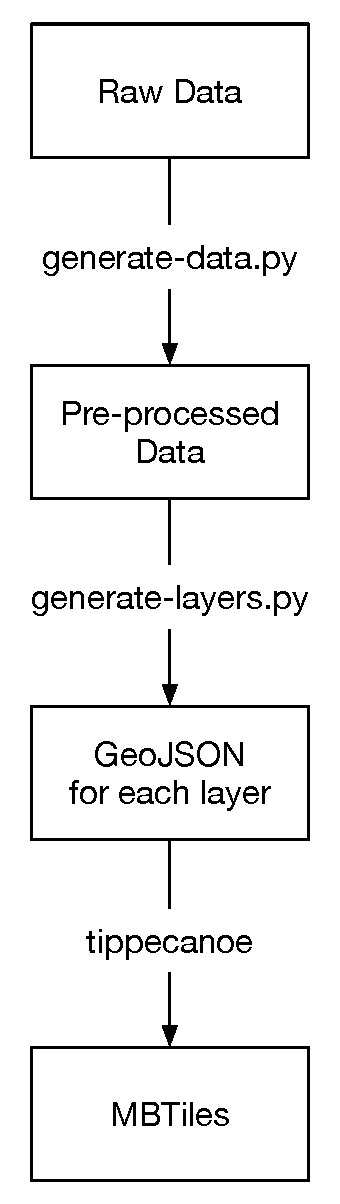
\includegraphics[width=.25\textwidth]{data-transformation.pdf}
  \caption{The process of the data transformation.}
  \label{pic:transforming_data}
\end{figure}

% ---
% Client
% ---
\subsection{Web Interface}

In this section the main architectural pattern used for building the interface is described
including diagrams showing hierarchy of components, the selection of map drawing library is made.

\subsubsection{FLUX Architecture}
In the process of the development of the web interface the crucial thing is the state management.
In 2010 the Backbone.js~\cite{backbone} library was introduced which was supposed to solve the problem of the
state management often applying MVC~\cite{backbone:mvc} pattern. Although, on large projects there
where a lot of cross-dependencies this paradigm resulted to be hard to maintain. Later in 2013
Facebook~Inc. introduced component based React~\cite{react} library, which allowed to think
of the interface as function which maps state to representation. Although, React was implemented
only as library for creating views and was not meant to solve problem of data state management in
the application it still had significant success. In 2014 Facebook~Inc. suggested FLUX~\cite{flux} pattern
which gained significant popularity. The idea behind FLUX can be described as follows: data comes
from the store to the view which renders it, the user can fire an action, for example by pressing
a button, the action is goes to the dispatcher which tells to all of the stores that certain action
was fired. The stores modify the data and broadcast it to all of the views which are subscribed to
this store. All of the views that received new data gets re-rendered. The illustration of this
process can be seen on Figure~\ref{pic:flux}.

\begin{figure}[h]
  \centering
  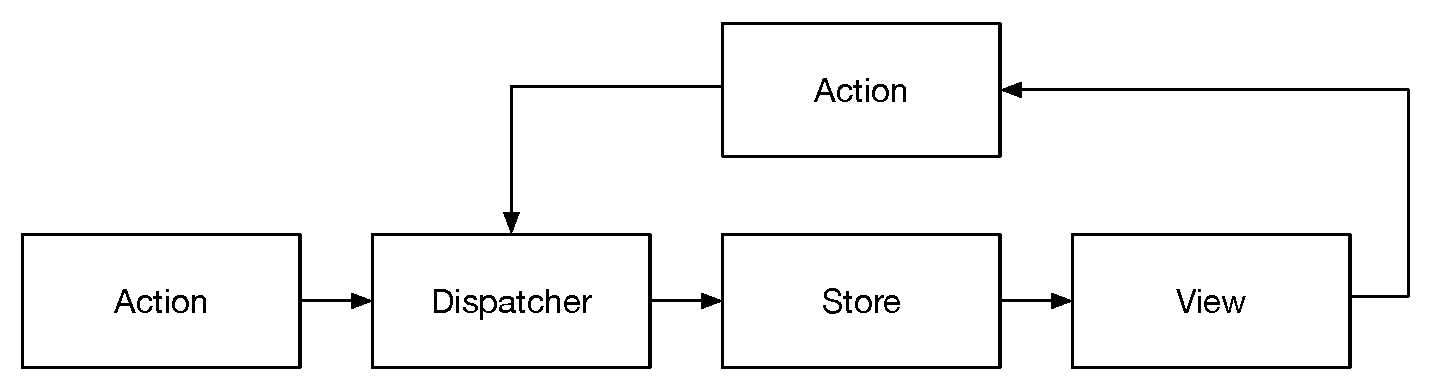
\includegraphics[width=.8\textwidth]{flux.pdf}
  \caption{FLUX architecture.}
  \label{pic:flux}
\end{figure}

Eventually FLUX evolved in library called Redux~\cite{redux}, which introduced few important
modifications such as suppressing dispatcher, using pure functions for data modifications, using
only single store where all of the data is accumulated, introducing middlewares for managing
side effects. All this features create easier debugging experience and clear separation
of concerns. Thus, for the development Redux and React libraries were chosen.

React components were organized accordingly to Figure~\ref{pic:comp-diag} accordingly to
the approach of presentational and container components~\cite{redux:ppc}. The main presentational
component is \texttt{App} which is the only one connected to the store directly. All other
components are ``dumb'' and receive data as well as actions which are
needed to be fired from \texttt{App}. The \texttt{SpeedMapButton} represents a switch for choosing
between coloring lines by speed and by the type of transport. The \texttt{Map} components
accumulates all of the logic related to drawing maps. The \texttt{TransportFilter} shows
what kind of transport should be displayed on the map. The \texttt{LocationSelector}
shows information about selected location. The \texttt{ModeSelector} switches between
global overview and location information. The positioning of all of the components is illustrated
by Figure~\ref{pic:comp-screen}.


\begin{figure}[ht]
  \centering
  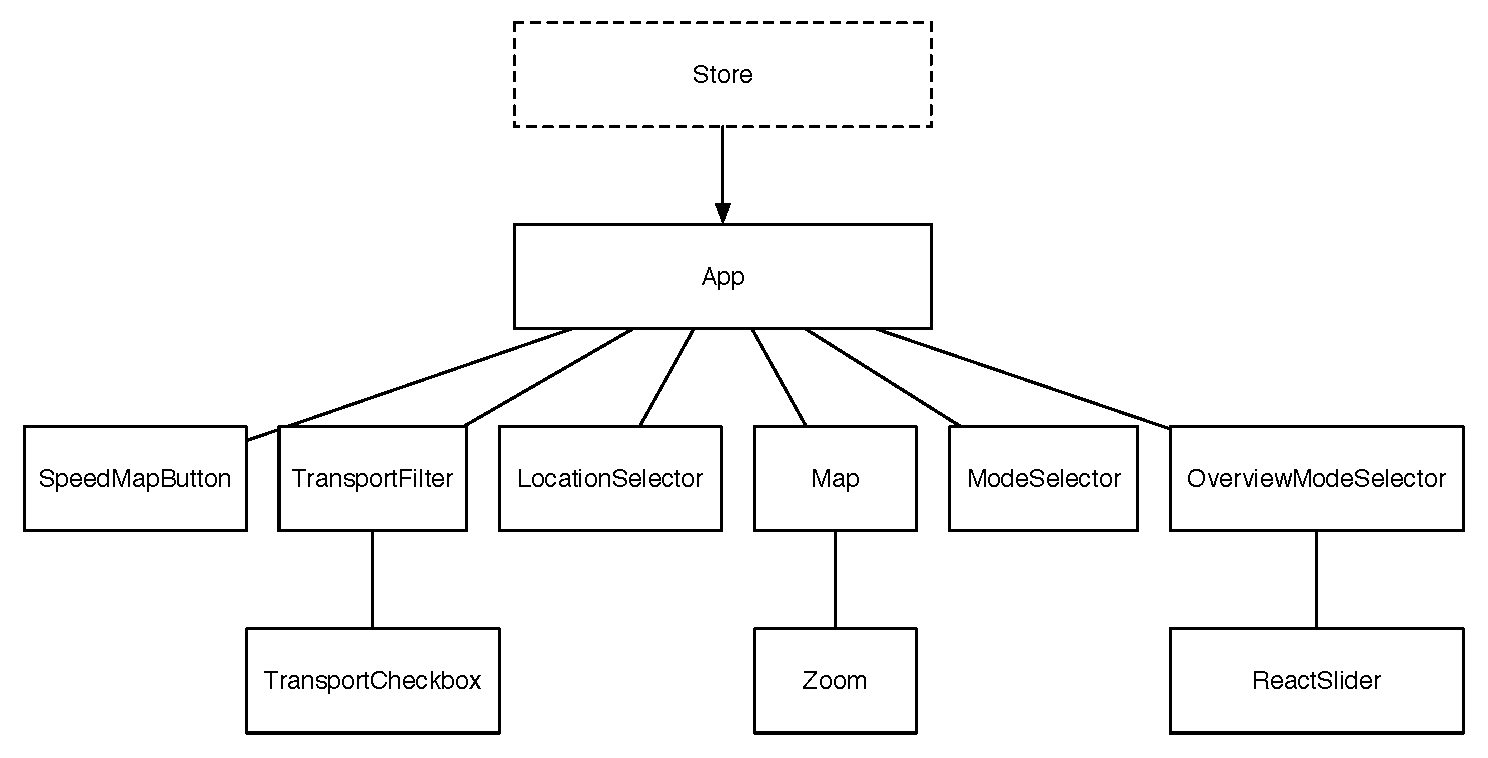
\includegraphics[width=1\textwidth]{components.pdf}
  \caption{Structure of the components}
  \label{pic:comp-diag}
\end{figure}

\begin{figure}[ht]
  \captionsetup{justification=centering,margin=1cm}
  \centering
  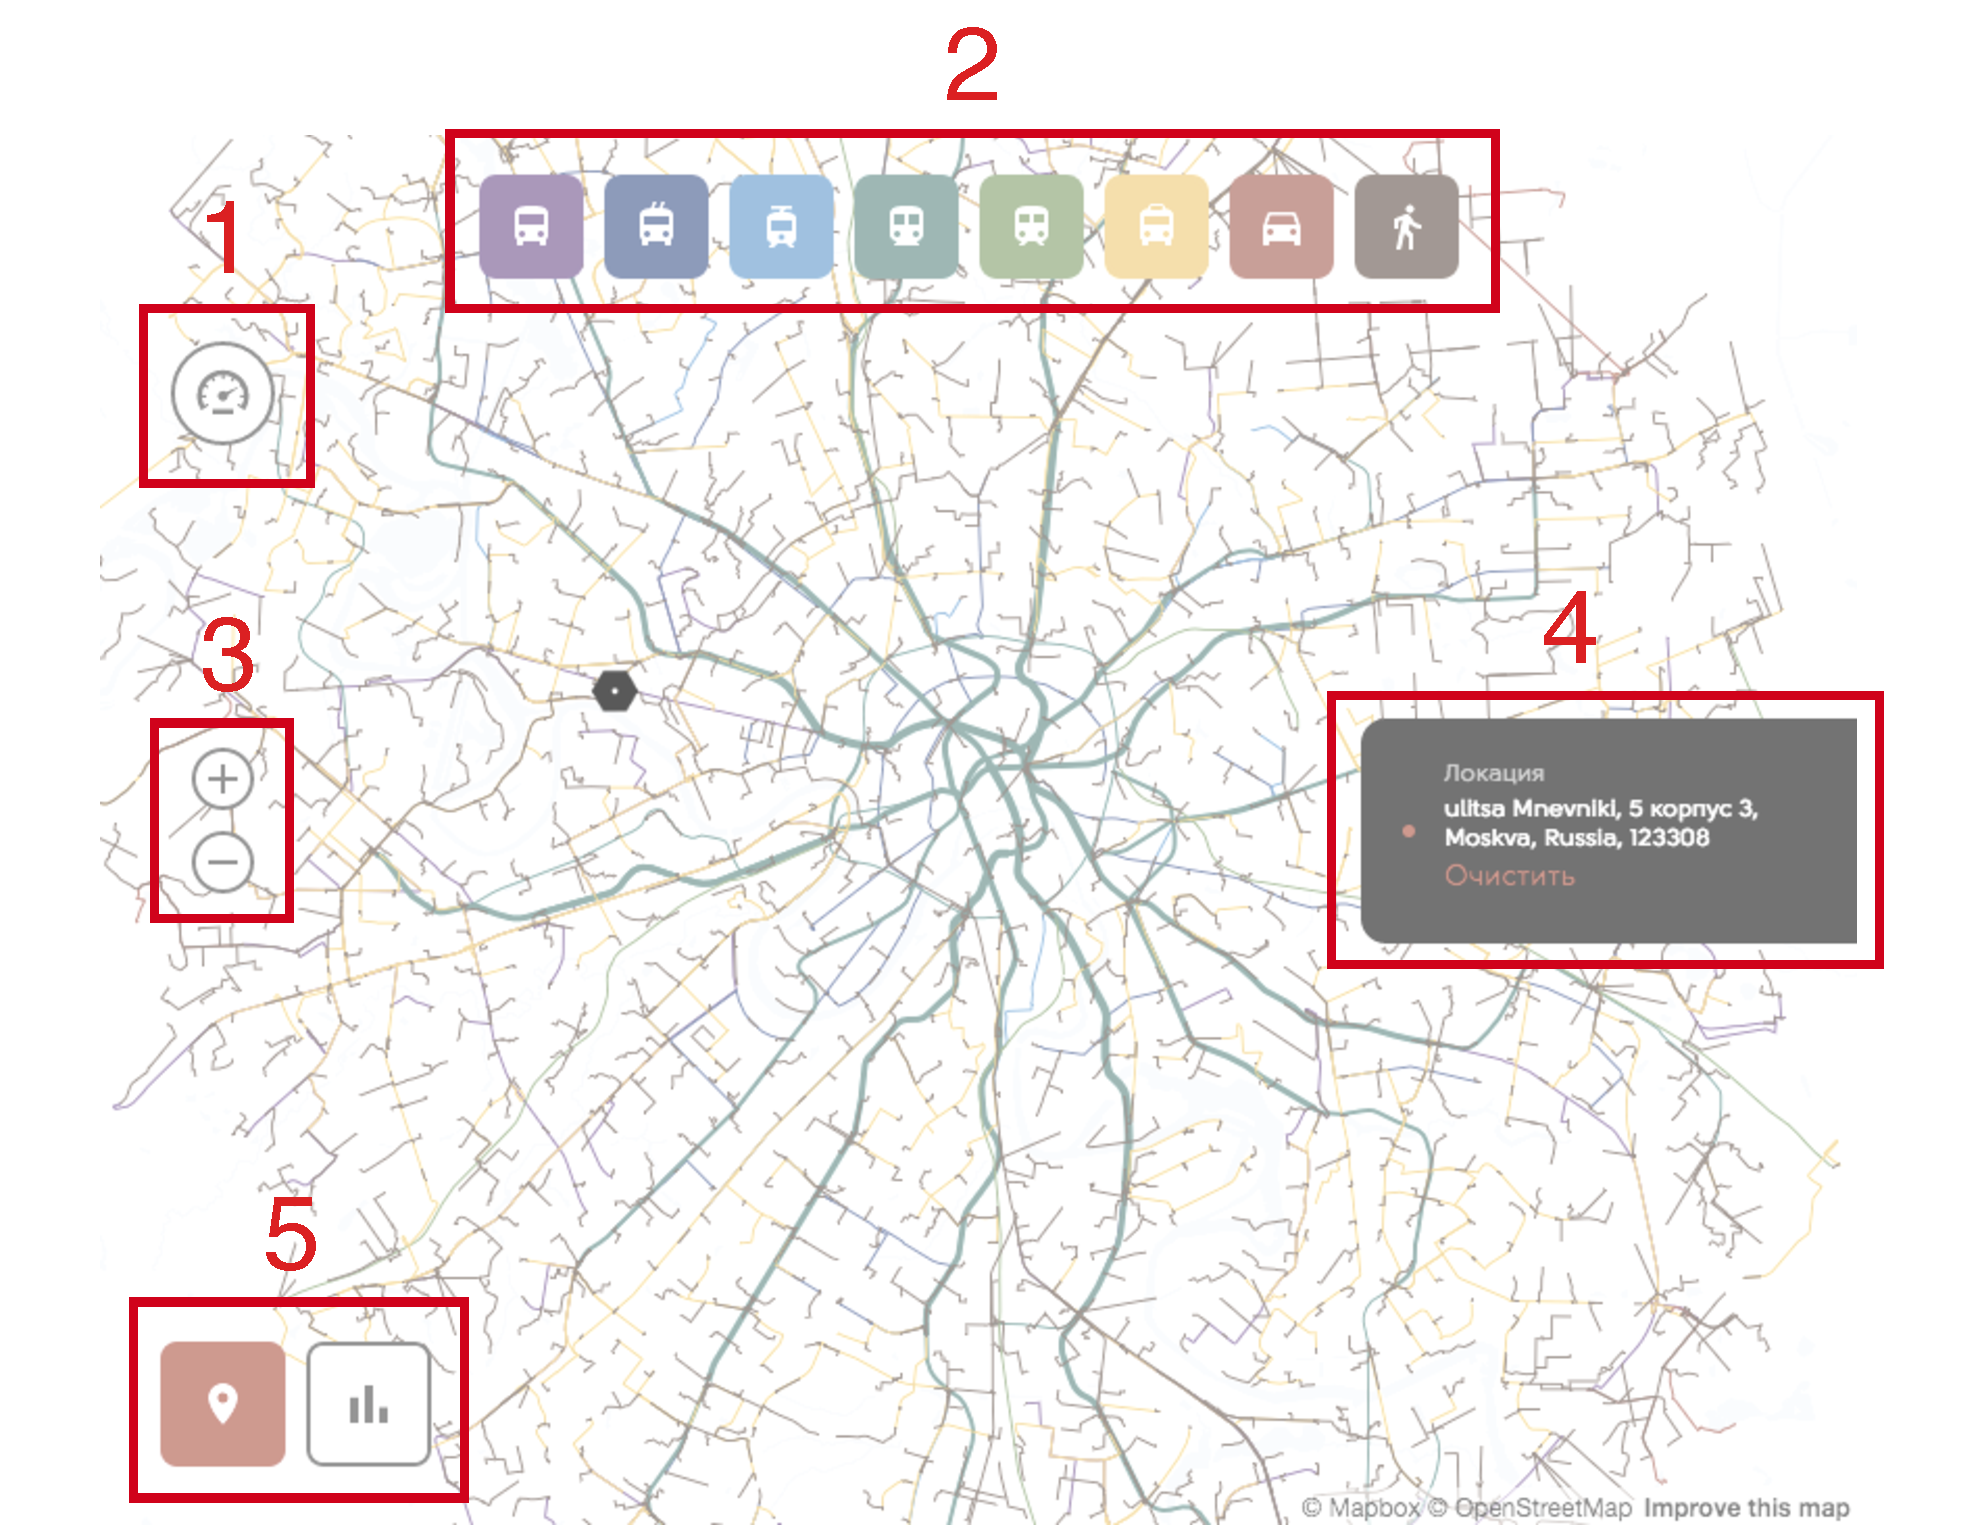
\includegraphics[width=.6\textwidth]{components-1.pdf}

  \par \vspace{0.5cm}

  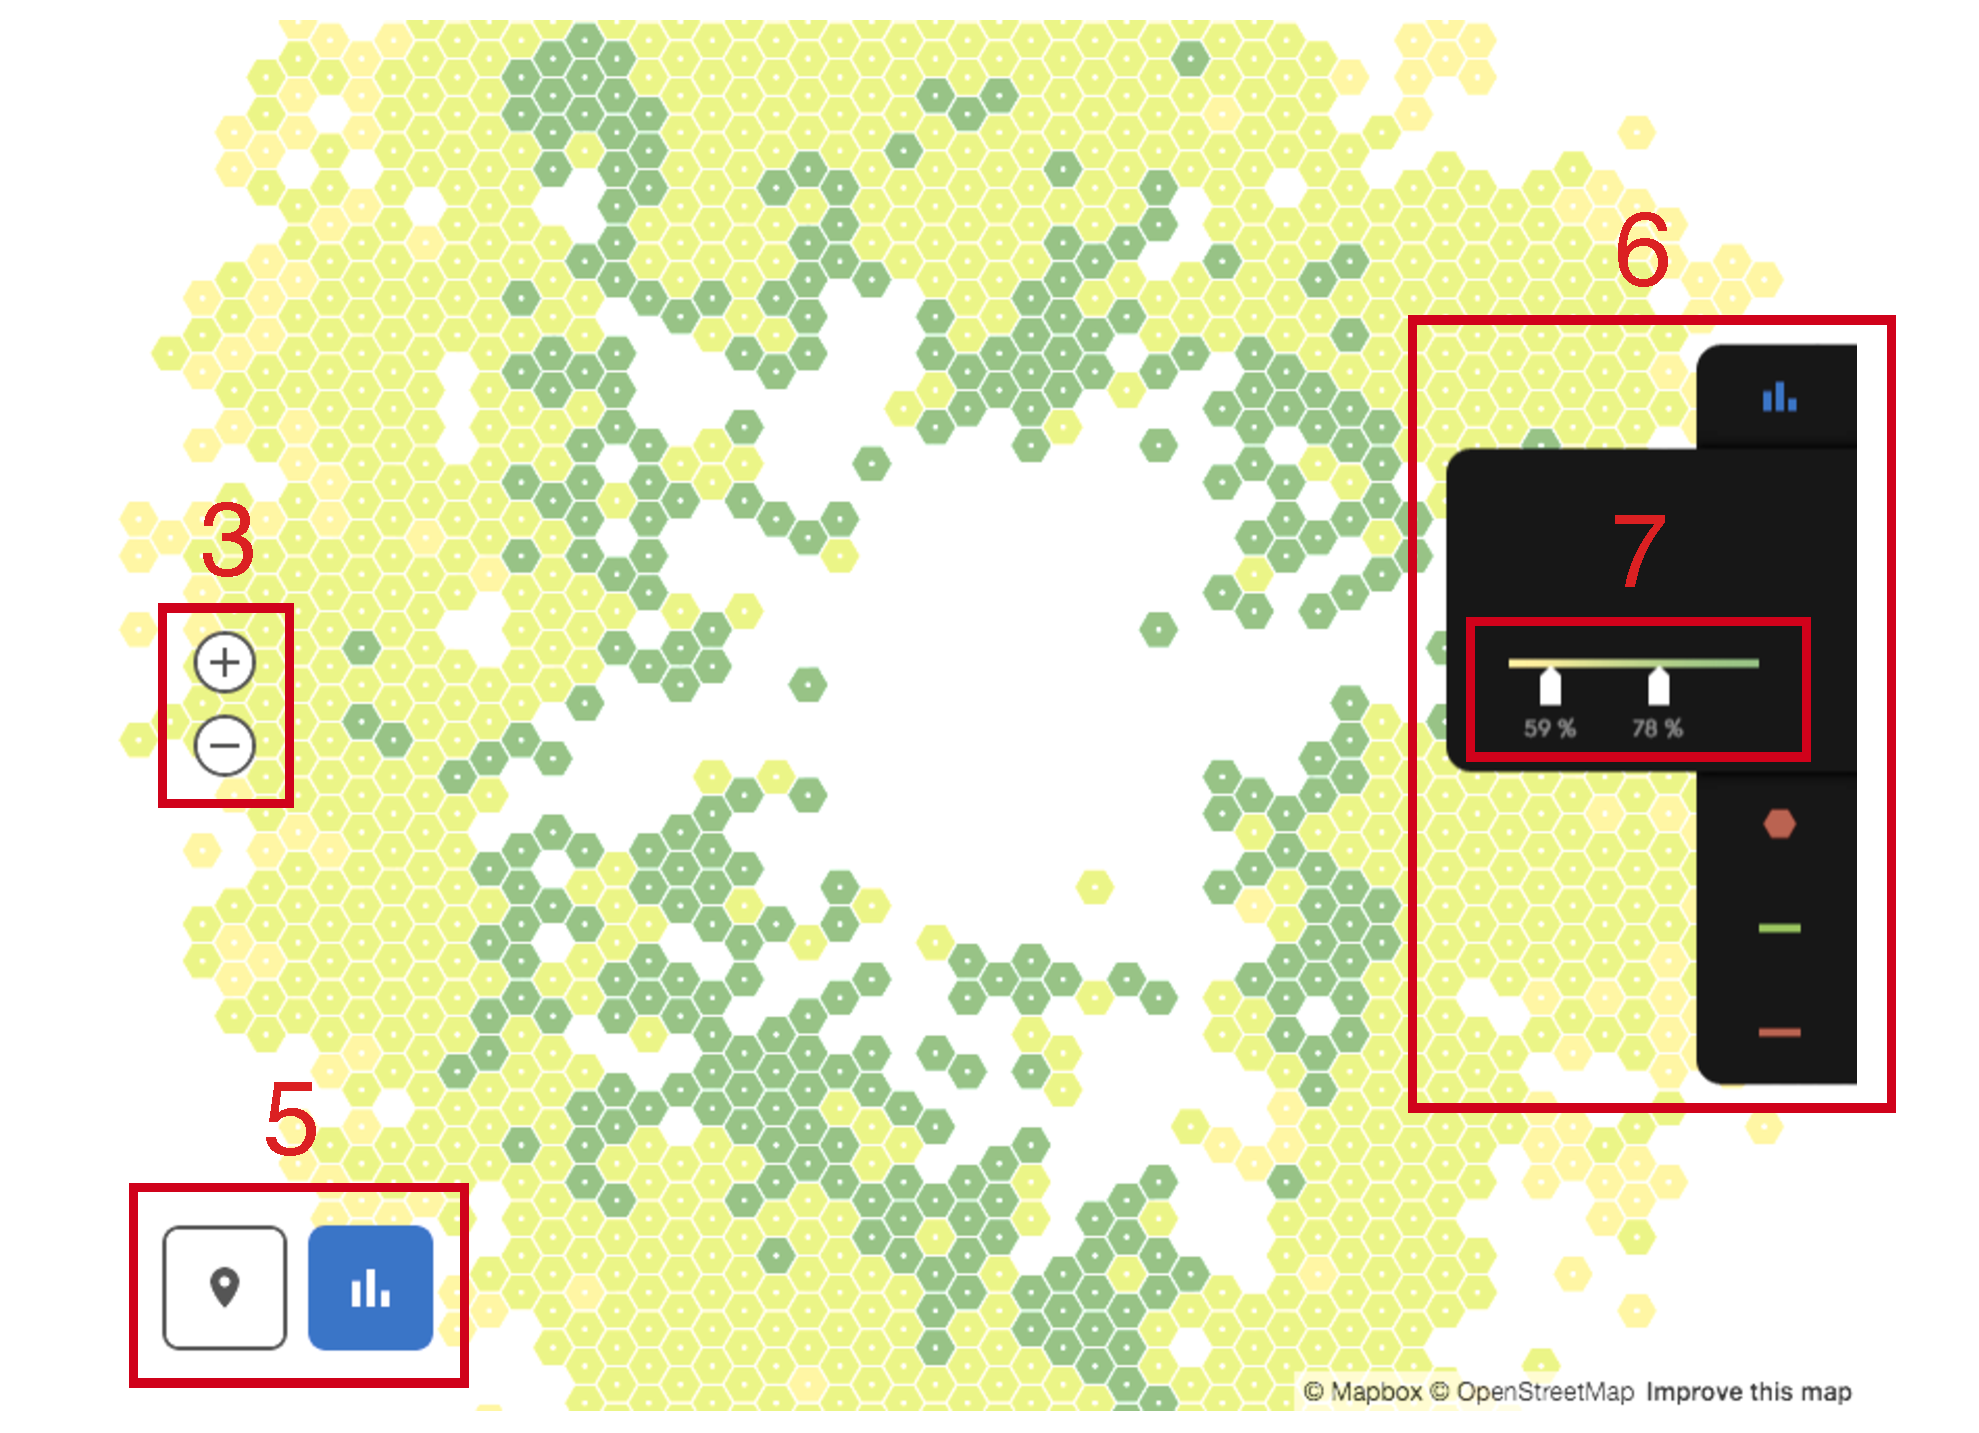
\includegraphics[width=.6\textwidth]{components-2.pdf}
  \caption{Components positioning. 1 -- SpeedMapButton; 2 -- TransportFilter; 3 -- Zoom;
  4 -- LocationSelector; 5 -- ModeSelector; 6 -- OverviewModeSelector; 7 -- ReactSlider.
  }
  \label{pic:comp-screen}
\end{figure}


\subsubsection{Drawing Maps}

As it was described before there are several the most famous libraries for drawing maps
such as Yandex Mapx, Google Maps, Leaflet.js and Mapbox GL JS. To determine which library will
suite better for our program, the needed functionality should be defined. The most important
features are:

\begin{enumerate}
  \item Panning and zooming.
  \item Support vector tiles.
  \item Rendering map from external data source.
  \item Support of the vector tiles styling of such properties as line widths, line colors.
  \item Ability to render icons at certain location.
  \item Support for map styling.
  \item Uses open standards.
\end{enumerate}

Among all of the libraries the most suitable is Mapbox GL JS which supports all of the listed features.
Although some part of the free Mapbox toolkit has limitations, for example free subscription
plan allows not more than 50000 map views per month, but for our project that was enough.
Important to note that Mapbox uses OpenStreeMap for geographical data provider which is
free to use.
As for Google Maps and Yandex Maps, they were not supporting maps from external data sources which
is needed for rendering custom vector tiles.
Although Leaflet is a very popular choice for map drawing, it is not suitable for our particular
application since it does not support vector tiles rendering.

\subsection{Tile Server}

For rendering all of the directions the tile server would need to be chosen. The tasks
in our application for this component are quite trivial:

\begin{enumerate}
  \item Fast.
  \item Support of the MBTiles format.
  \item Easy to setup and configure.
  \item Free and open-source.
\end{enumerate}

The great candidate for this role was Tessera tile server~\cite{gh:tessera} which is written in
Node.js and based on Tilelive interface (developed by Mapbox). Moreover, Tessera
is really easy to install using npm package manager. The configuration file should be
written in JSON format and can be easily generated from our data. The only needed parameters
are source path to the data and the URL on which particular vector tiles will be available.
%!TEX root = ../thesis.tex
\section{INTEGRATION}

One of the important aspects of the development process is the set of tools which were
used. In this section the particular methods and tools will be described, which
were applied on course of making this program. Another part will be devoted to
the deployment.

\subsection{Development Environment}

Right set of tools can significantly speed up development process by lowering probability of making
an error, provide extensions to the language which may help to structure code for higher
maintainability. In out project, tools may be split into two categories, namely client-side and
server-side utilities.

When JavaScript was used for simple interactions on the HTML page, the development of the client
code was quite straight-forward: create \texttt{.js} file, write some code, include the script to
the index.html. Unfortunately, when applications started to become more complex it was clear that
code had to be split into reusable modules. This problem was solved in ES2015 JavaScript standard
[REFERENCE] which introduced the concept of modules, however, now only small percent of the browsers
support new standard. To solve the problem with compatibility the Webpack was chosen. Webpack is a
module bundler which allows split the code into different files. Once the project would need to
built webpack is going through all of the imports and packing all modules in one solid bundle which
can be easily included into HTML page.

One of the core concepts of the webpack is loaders. Loader is a transformation
of the file. There are pre-installed loaders such as JavaScript loader for
bundling JavaScript files together. Loaders can be chained, allowing to use modern
JavaScript syntax that can be transformed to normal JavaScript. Webpack
works not only with JavaScript, but also with CSS so it becomes possible to include
CSS files in JavaScript and use plug-ins like ``autoprefixer'' to write cleaner styles.

It is a common problem when different project use different versions of the same
package. To overcome this issue on the server the pyenv was used. Pyenv allows
to create virtual environment where you can locally install all needed packages. Virtual
environments are completely isolated which illuminates the problem of the dependencies version
conflict.

\subsection{Deploying the Project}

To quickly run project in development environment the make tool was used. There is a Makefile
which runs all needed commands to start up three servers on different ports. However,
to run project on remote server four steps need to be performed:

\begin{enumerate}
  \item Install all dependencies.
  \item Build client code.
  \item Install proxy server such nginx [REFERENCE] and wire up tile server and API server ports with it.
  \item Setup nginx for serving statics (HTML, JavaScript and assets) on 80 port.
  \item Start the tile server and the API server.
\end{enumerate}
%!TEX root = ../thesis.tex
\section{CONCLUSION}

The system for transport accessibility analysis of Moscow was developed, which allows to explore
regions of the city. The program allows to browse locations and see examine what are the most
used roads when traveling from particular region to all other locations of the city. The service
provides global overview of the city in terms of prevailing transport for each region, fastest
and slowest roads. Accessibility level is calculated for each region, allowing to filter and
discover most accessible and least accessible parts of the city.

The software is developed applying cutting-edge techniques in web development which resulted
in highly responsive systems and helped to achieve insignificant delays. The reliability of the
system was proved by test driven development approach. All of the provided software requirements
were satisfied.

% ---
% Bibliography
% ---
\addcontentsline{toc}{section}{REFERENCES}
\bibliography{bibliography/references}

\end{document}
